\documentclass{article}

\usepackage{amsmath}
\usepackage{listings}
\usepackage{graphicx}


\title{Data Analysis and Visualisation using R}
\date{2016-01-11}
\author{\textbf{Wing Cheung Kenneth Lui} \\
Computer Laboratory, University of Cambridge \\
{\tt wckl2@cam.ac.uk}}

\begin{document}
  \pagenumbering{arabic}
  \maketitle

\section{Introduction}

In this study, we analyse a training dataset provided in CSV (comma-separated values) format. There are 1800 observations (i.e. rows) and 12 columns of values in total. The first column, named {\tt id}, contains unique integer identifiers from 1 to 1800; the second column, named {\tt Y}, stores a number without containing any {\tt NA} values; {\tt Y} is followed by nine floating point numeric columns named from {\tt X1}, {\tt X2},  \(...\), {\tt X9}, which may contain {\tt NA}s in some observations; finally, the last column, named {\tt label}, contains one of eight text values such as ash, beech, oak and so on.

We divide the data into eight uneven subsets based on the label value. During preprocessing, {\tt id}, {\tt label} and {\tt NA} entries are removed from each subset. The number of observations and the remaining column names is tabulated in Table~\ref{subset-table}. In statistical learning context, the training data are observations where the response variable Y may have some relationship with one or more of the potential predictor variables {\tt X\textsubscript{i}}.

\begin{table}
\begin{center}
\begin{tabular}{|c|c|c|}
\hline \bf Label & \bf Number of observations & \bf Predictor variables \\ \hline
ash & 500 & {\tt X1, X2, X3, X4, X5, X6, X7, X8, X9} \\ \hline
beech & 500 & {\tt X3, X7} \\ \hline
elder & 500 & {\tt X7} \\ \hline
elm & 100 & {\tt X3, X8} \\ \hline
larch & 50 & {\tt X3, X4, X5, X9} \\ \hline
oak & 50 & {\tt X3} \\ \hline
rowan & 50 & {\tt X4} \\ \hline
yew & 50 & {\tt X4} \\ \hline
\end{tabular}
\end{center}
\caption{\label{subset-table} Overview of subset in training data.}
\end{table}

\section{Statistical Analyses}

A variety of regression and classification techniques have been employed to detect characteristics and dependencies underlying the training data. The results are presented graphically and numerically in this report.

\begin{table}
\begin{center}
\begin{tabular}{|c|c|}
\hline \bf Library & \bf Functions provided \\ \hline
{\textit class} & {\tt knn(), cv.knn()} \\ \hline
{\textit leaps} & {\tt regsubsets()} \\ \hline
{\textit MASS} & {\tt lda(), qda()} \\ \hline
\end{tabular}
\end{center}
\caption{\label{library-table} Overview of libraries used.}
\end{table}

\subsection{Ash subset}

The response variable {\tt Y} is continuous so regression methods are used. First, we use {\tt pairs()} to produce a matrix of pairwise scatterplots for each pair of variables ({\tt Y} and all {\tt X\textsubscript{i}}) to detect whether any observable patterns exist. {\tt X7} shows an obvious linear relationship with {\tt Y} in these plots so we use {\tt lm()} to fit a \textbf{simple linear regression} between them. The summary of this fit shows that the least squares coefficients of {\tt X7} in the linear relationship is highly significant (p-value is close to zero). Its training $R^2$ value of 0.9966 shows that the variance left unexplained by the linear fit is negligible. This fit also results in a convincing inspection plot as shown in Figure~\ref{fig:01-ash}. No obvious pattern can seen in the residuals vs fitted values plot. However, this should not rule out the possibility that {\tt Y} is also related to some other predictors. we perform a \textbf{multiple linear regression} using all available predictors and obtain an ``improved'' fit where both {\tt X3} and {\tt X7} are significant and training $R^2$ value is 0.9988. But such improvement must be taken with a grain of salt because {\em training $R^2$ values for any more flexible models (i.e. those with more predictors) must be no less than a more restrictive one}. To verify whether a simple linear model involving {\tt X7} only is the true relationship over other more flexible multiple linear models, 5-fold cross-validation has been used with best subset variables selection. As shown in Listing~\ref{ash}, cross-validation suggests $Y \sim X3+X4+X7+X8$ as the model achieving the lowest test squared error but the performance difference compared to $Y \sim X3$ is small, which is chosen for the sake of interpretability.

\begin{figure}[h!]
  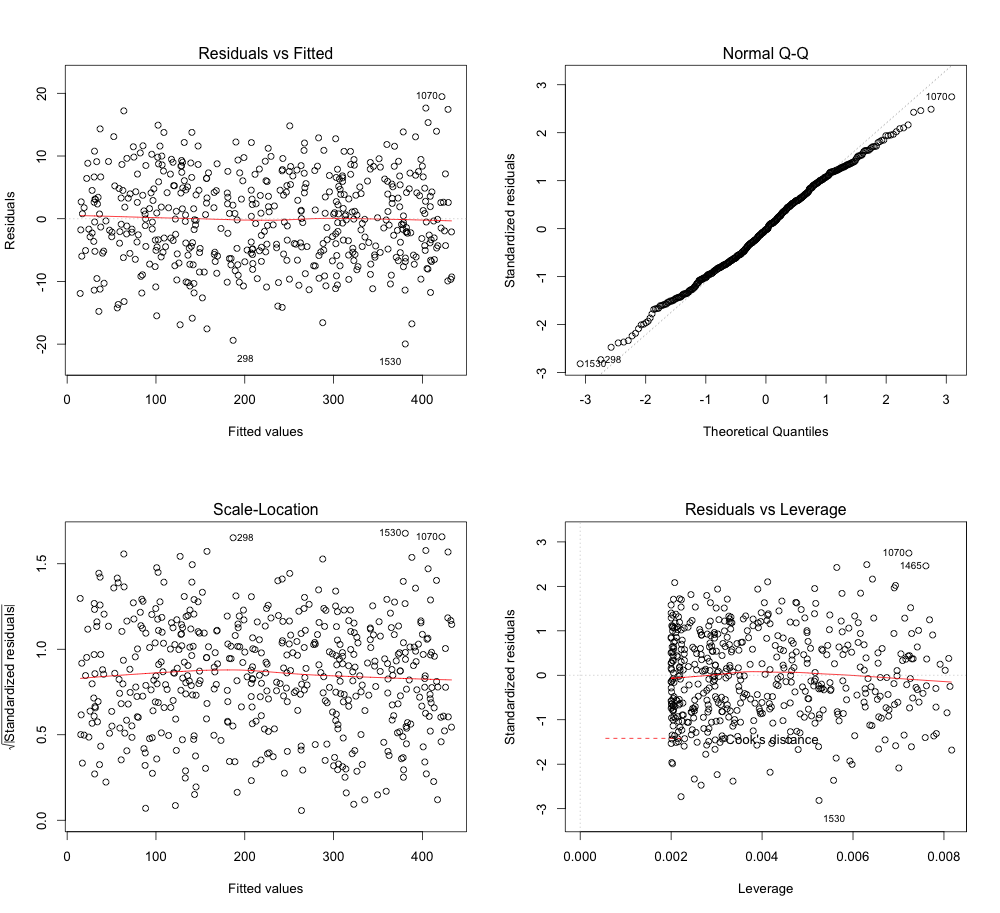
\includegraphics[width=\linewidth]{project/images/01-ash.png}
  \caption{Inspection plots for linear fit $Y \sim X7$ in ash dataset.}
  \label{fig:01-ash}
\end{figure}

\subsection{Beech subset}

We approach the problem from a classification perspective because the response variable Y is binary (either 0 or 1). In a binary classification problem, it is helpful to plot all the data points on the same scatter plot using distinct symbols to visualise how the two classes are separated, as shown in Figure~\ref{fig:02-beech}. While the separation between the two classes is not absolutely clear, the boundary seems to be linear rather than quadratic. We first randomly divide the data into a training set and a test set so we can quantitatively compare models given by  \textbf{logistic regression},  \textbf{linear discriminant analysis (LDA)} and  \textbf{quadratic discriminant analysis (QDA)}. These three methods achieve test classification accuracies at 89.6\%, 90.8\% and 89.6\% respectively. This result suggests that the class boundary is linear, so the flexibility ``gained'' by using QDA is not useful to offset the extra errors caused by {\em variability} in the model. While both logistic regression and LDA model a linear boundary, LDA's slight performance gain over logistic regression may be explained by LDA's assumption. Its assumption states that predictors are drawn from a multivariate Gaussian distribution with a class-specific mean vector and a common covariance matrix. By inspecting the mean vector and covariance matrix computed for each class, LDA's assumption appears to be correct on this training data set. We also experiment with \textbf{k-Nearest Neighbors (KNN)} classification but it does not give significantly different results.

\begin{figure}[h!]
  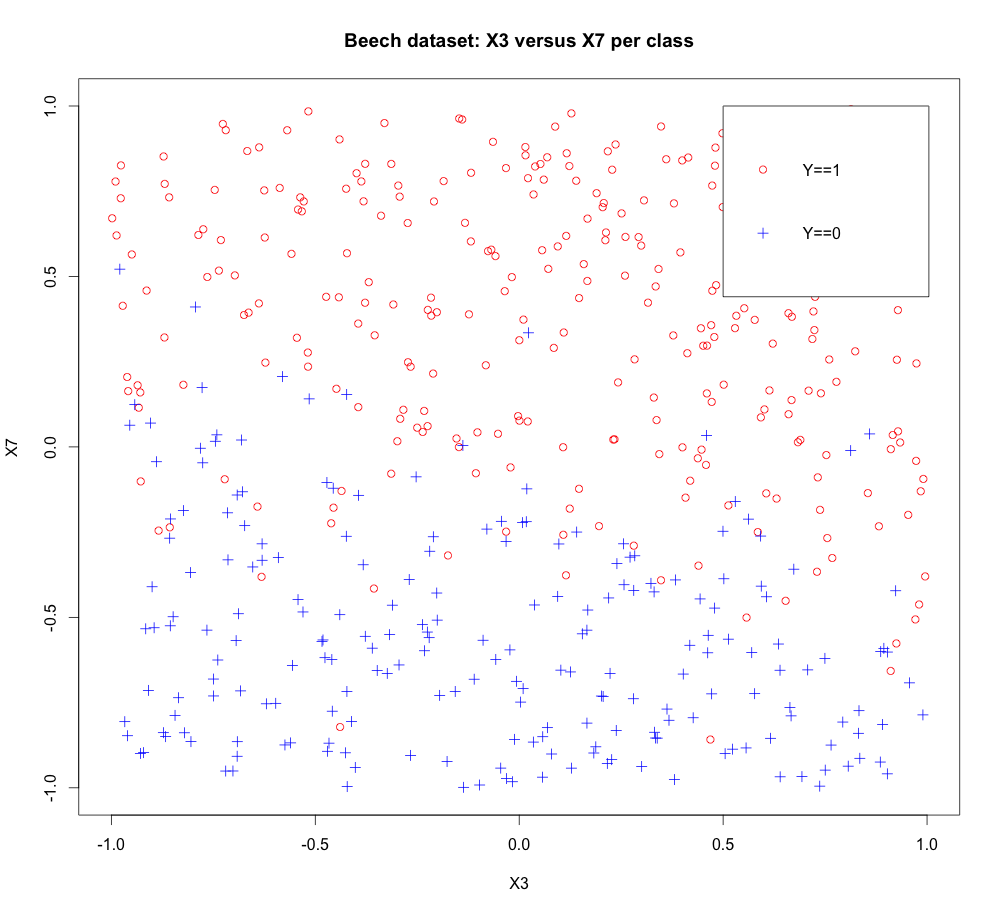
\includegraphics[width=\linewidth]{project/images/02-beech.png}
  \caption{Inspection plot for decision boundary in beech dataset.}
  \label{fig:01-beech}
\end{figure}

\subsection{Elder subset}

We start exploring this set of data by plotting a scatterplot between {\tt Y} and {\tt X7}, the only remaining predictor. We observe that a funnel shape formed by the data points overshadows an upward linear relationship, as shown in Figure~\ref{fig:03-elder}. The funnel shape may imply a non-constant variance in the error terms, a phenomenon called {\em heteroscedasticity}. In this data set, heteroscedasticity causes the variance in error terms increases with the response values. One possible solution is transforming the response variable using a concave function hence we compare three models: $Y \sim X7$, $log(Y) \sim X7$ and $\sqrt{Y} \sim X7$. The funnel-shaped pattern and magnitude observed in the residuals versus fitted values plot for the simple linear regression model has been greatly reduced in Figure~\ref{fig:04-elder}, although not completely eliminated, through the use of concave transformation. The training $R^2$ values for these models are 0.3359, 0.3305 and 0.3373 respectively. Based on this, we have chosen $sqrt{Y} \sim X7$ as the resulting linear regression coefficients are significant.

\begin{figure}[h!]
  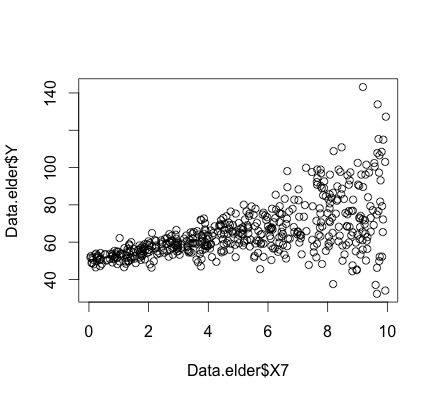
\includegraphics[width=\linewidth]{project/images/03-elder.png}
  \caption{Inspection plot for heteroscedasticity in elder dataset.}
  \label{fig:03-elder}
\end{figure}

\begin{figure}[h!]
  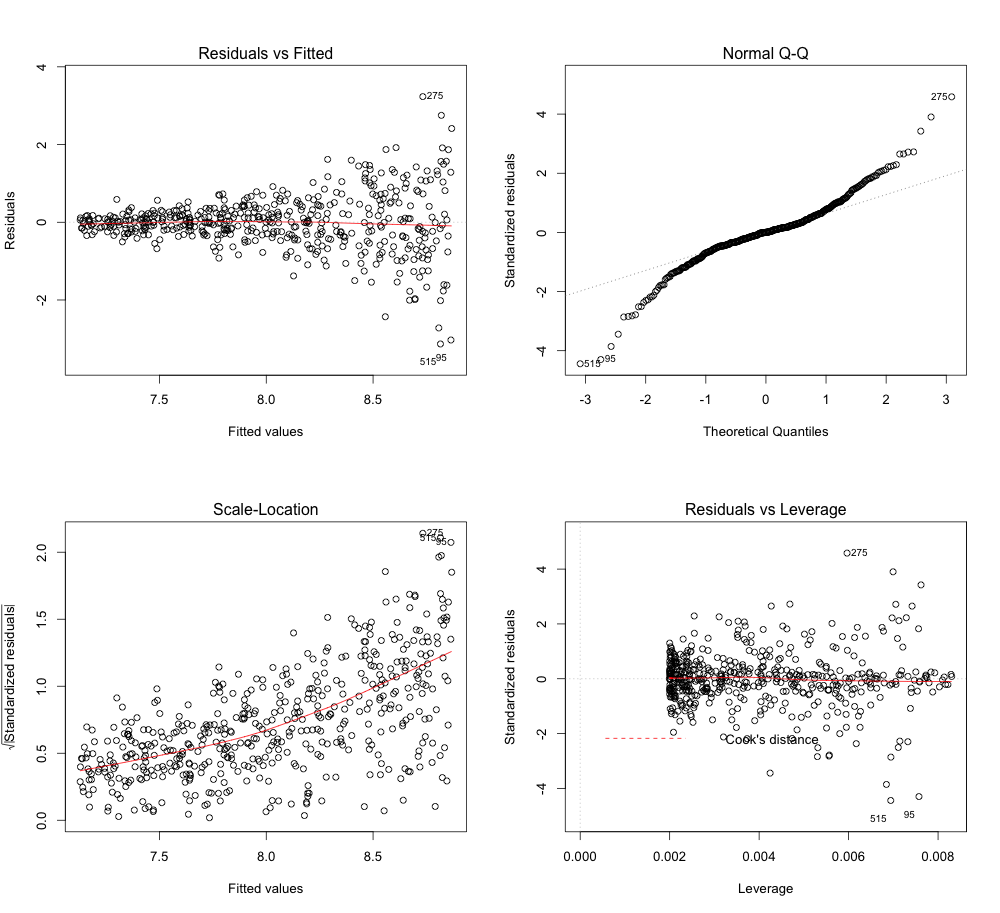
\includegraphics[width=\linewidth]{project/images/04-elder.png}
  \caption{Inspection plots showing reduced funnel-shape residuals for $\sqrt{Y} \sim X7$ in elder dataset.}
  \label{fig:04-elder}
\end{figure}

\subsection{Elm subset}

Since the response variable Y is qualitative (represented in 0 or 1), we perform classification analysis similar to the beech subset. A difference noticeable by inspecting the scatter plot (Figure~\ref{fig:05-elm}) is that the two classes are more well-separated in this data set compared to the beech subset. We follow the same approach, divide the data into a training set and a test set, then apply logistic regression, LDA and QDA to the training set. Surprisingly, these three methods give the exact same prediction for the test set and their prediction accuracy is 90.2\% on the test set. On the other hand, it may be interesting to compare these three parametric methods with a non-parametric method, namely k-nearest neighbour (KNN). Before applying KNN, the predictors should be {\em standardized} to have zero mean and unit variance. we perform three KNN predictions on the standardized data with {\tt K}=1, 3 and 10. A larger K, which specifies the number of nearest neighbour to be considered, implies less variance in the model and higher bias. Despite this conceptual bias-variance trade-off, we achieve exactly the same 87.8\% prediction accuracy rate on the test set regardless of our choice of {\tt K}. The predictions given by {\tt K}=1 and {\tt K}=3 are exactly the same and they are different from {\tt K}=10 by two predictions. we think the parametric methods outperform the non-parametric KNN method because the underlying classification boundary is linear so a simpler model is less prone to noise in the data. The flexibility of KNN method is an overkill and does not cause a comparative advantage.

\begin{figure}[h!]
  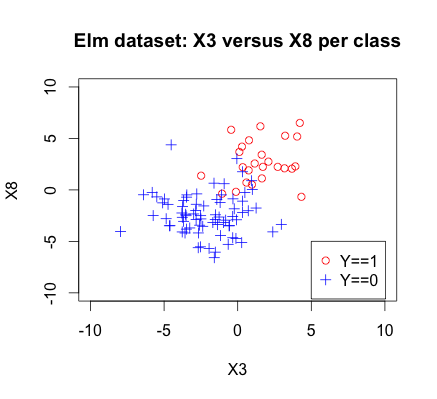
\includegraphics[width=\linewidth]{project/images/05-elm.png}
  \caption{Inspection plot for decision boundary in elm dataset.}
  \label{fig:05-elm}
\end{figure}

\newpage

\paragraph{Appendices}

\lstinputlisting[breaklines=true,language=R,caption={sharecode.R},label=sharedcode]{project/1-sharedcode.R}

\rule{\textwidth}{1pt}

\lstinputlisting[breaklines=true,language=R,caption={preprocessing.R},label=preprocessing]{project/2-preprocessing.R}

\rule{\textwidth}{1pt}

\newpage

\lstinputlisting[breaklines=true,language=R,caption={ash.R},label=ash]{project/3-ash.R}

\rule{\textwidth}{1pt}

\lstinputlisting[breaklines=true,language=R,caption={beech.R},label=beech]{project/4-beech.R}

\rule{\textwidth}{1pt}

\lstinputlisting[breaklines=true,language=R,caption={elder.R},label=elder]{project/5-elder.R}

\rule{\textwidth}{1pt}

\lstinputlisting[breaklines=true,language=R,caption={elm.R},label=elm]{project/6-elm.R}

\rule{\textwidth}{1pt}

\lstinputlisting[breaklines=true,language=R,caption={larch.R},label=larch]{project/7-larch.R}

\rule{\textwidth}{1pt}

\lstinputlisting[breaklines=true,language=R,caption={oak.R},label=oak]{project/8-oak.R}

\rule{\textwidth}{1pt}

\lstinputlisting[breaklines=true,language=R,caption={rowan.R},label=rowan]{project/9-rowan.R}

\rule{\textwidth}{1pt}

\lstinputlisting[breaklines=true,language=R,caption={yew.R},label=yew]{project/10-yew.R}

\rule{\textwidth}{1pt}

\end{document}